\section{Benchmark}
\label{sec:benchmark}

We introduce a benchmark for \emph{Socially-Aware Audio-Visual Navigation} (SAVNav), in which an embodied agent must navigate to a semantic acoustic target while interpreting ambient human sounds as dynamic social constraints. Unlike conventional audio-visual navigation, which treats sound merely as a goal, and unlike vision-based social navigation, which reasons only about visible humans, SAVNav requires the robot to jointly reason about \emph{task-relevant acoustic targets} and \emph{socially meaningful acoustic boundaries}. 

\subsection{Task Definition and Scenario Families}
\label{subsec:benchmark-task}

Each episode is defined by an indoor scene, a robot start state, a language query $q$ specifying the acoustic target (chosen from \texttt{doorbell}, \texttt{calling} (a person verbally summoning the robot), \texttt{music}, \texttt{running water}), and a set of human agents. The robot must navigate to the target source. Crucially, the environment also contains humans who may emit social sounds (\texttt{chat}, \texttt{footstep}), which act as dynamic obstacles or social zones that the robot must not intrude upon.

To rigorously evaluate the agent's capabilities across different physical and social contexts, we structure the benchmark into three distinct \emph{Scenario Families}. Rather than relying on abstract difficulty grids, this taxonomy evaluates the robot's performance against realistic spatial challenges:

\begin{itemize}
    \item \textbf{Scene A: Crowded Social Scene.} A high-density, fully visible environment containing 3--5 humans. It features at least one \emph{Stationary Conversational Group} (SCG) and roaming individuals (\emph{Dynamic Pedestrians}, DP). The core challenge is navigating through tight, socially dense spaces without interrupting conversations or violating personal space.
    \item \textbf{Scene B: Hidden Boundary Scene.} Focuses on non-line-of-sight (NLOS) social risks. The scene contains a primary hidden actor completely occluded by geometry (e.g., around a blind corner or behind a door). It includes two variants: \emph{B1 (Hidden SCG)} testing the avoidance of unseen conversational zones, and \emph{B2 (Hidden DP)} testing early yielding to approaching pedestrians before visual contact. The core challenge is acoustic-to-spatial mapping (hearing before seeing).
    \item \textbf{Scene C: Mixed Home Activity.} A generalized, everyday domestic scenario featuring 2--3 humans with a mix of visible and invisible actors (e.g., one person visible in the living room, another walking in a hidden hallway). This ensures the benchmark evaluates robust, general-purpose navigation rather than merely overfitting to isolated stress tests.
\end{itemize}

\begin{table*}[t]
	\centering
	\caption{SAVNav Benchmark Scenario Families. The taxonomy explicitly isolates the challenges of visible social routing (Scene A) and NLOS acoustic anticipation (Scene B), while ensuring generalizability in composite environments (Scene C).}
	\label{tab:benchmark_tiers}
	\begin{tabular}{lccll}
		\toprule
		Scenario Family & Human Count & Human Visibility & Social Composition & Core Challenge \\
		\midrule
		\textbf{Scene A} (Crowded Social) & 3--5 & Visible & Mixed (SCG \& DPs) & Social routing and yielding in visually dense spaces. \\
		\textbf{Scene B} (Hidden Boundary)& 1--2 & NLOS    & Single (SCG or DP) & \textbf{Hearing before seeing}. \\
		\textbf{Scene C} (Mixed Home)     & 2--3 & Mixed   & Mixed (Visible \& NLOS) & Robust multi-modal attention and generalizability. \\
		\bottomrule
	\end{tabular}
\end{table*}

\subsection{Simulation and Episode Generation}
\label{subsec:benchmark-sim}

The benchmark is built upon a high-fidelity simulator that combines multi-agent human behaviors (Habitat 3.0) with physically grounded acoustic rendering (SoundSpaces 2.0). To ensure diverse and realistic interactions, we utilize large-scale indoor environments from the Matterport3D (MP3D) dataset. Episodes are strictly restricted to single-floor layouts with a limited number of interconnected regions ($\le 10$ rooms) to prevent ambiguous vertical sound propagation and unbounded exploration. Each episode allows a maximum of 600 time steps. We specifically select 10 diverse scenes to generate the evaluation dataset, comprising approximately 1,000 episodes distributed evenly across the three scenario families (Scenes A, B, and C).

To ensure episodes accurately reflect the scenario families, we enforce strict parametric settings during generation.

\textbf{Acoustic Configurations.} Each episode contains a maximum of 3 active sound sources: 1 target source and up to 2 social distractor sounds. For Scenes B and C, the presence of social sounds (\texttt{footstep} or \texttt{chat}) inevitably creates a complex acoustic mixture with the target audio. The agent must perform source separation rather than treating these social cues purely as noise.

\textbf{Spatial and Dynamic Settings.} For Scene A, humans are spawned within the main topological pathways to force spatial negotiation. For Scene B (NLOS), we use raycast initialization from the robot's starting pose to ensure the humans are strictly visually occluded. Furthermore, for dynamic humans (DP), we generate navigation waypoints such that their trajectory explicitly intersects with the robot's shortest geodesic path to the target. This forced-intersection design guarantees that the robot cannot succeed by simply ignoring the human; it must proactively yield or alter its path based on approaching footsteps.

\begin{figure}[t]
	\centering
	% TODO: replace with the finalized simulation figure showing the 3 scenes
	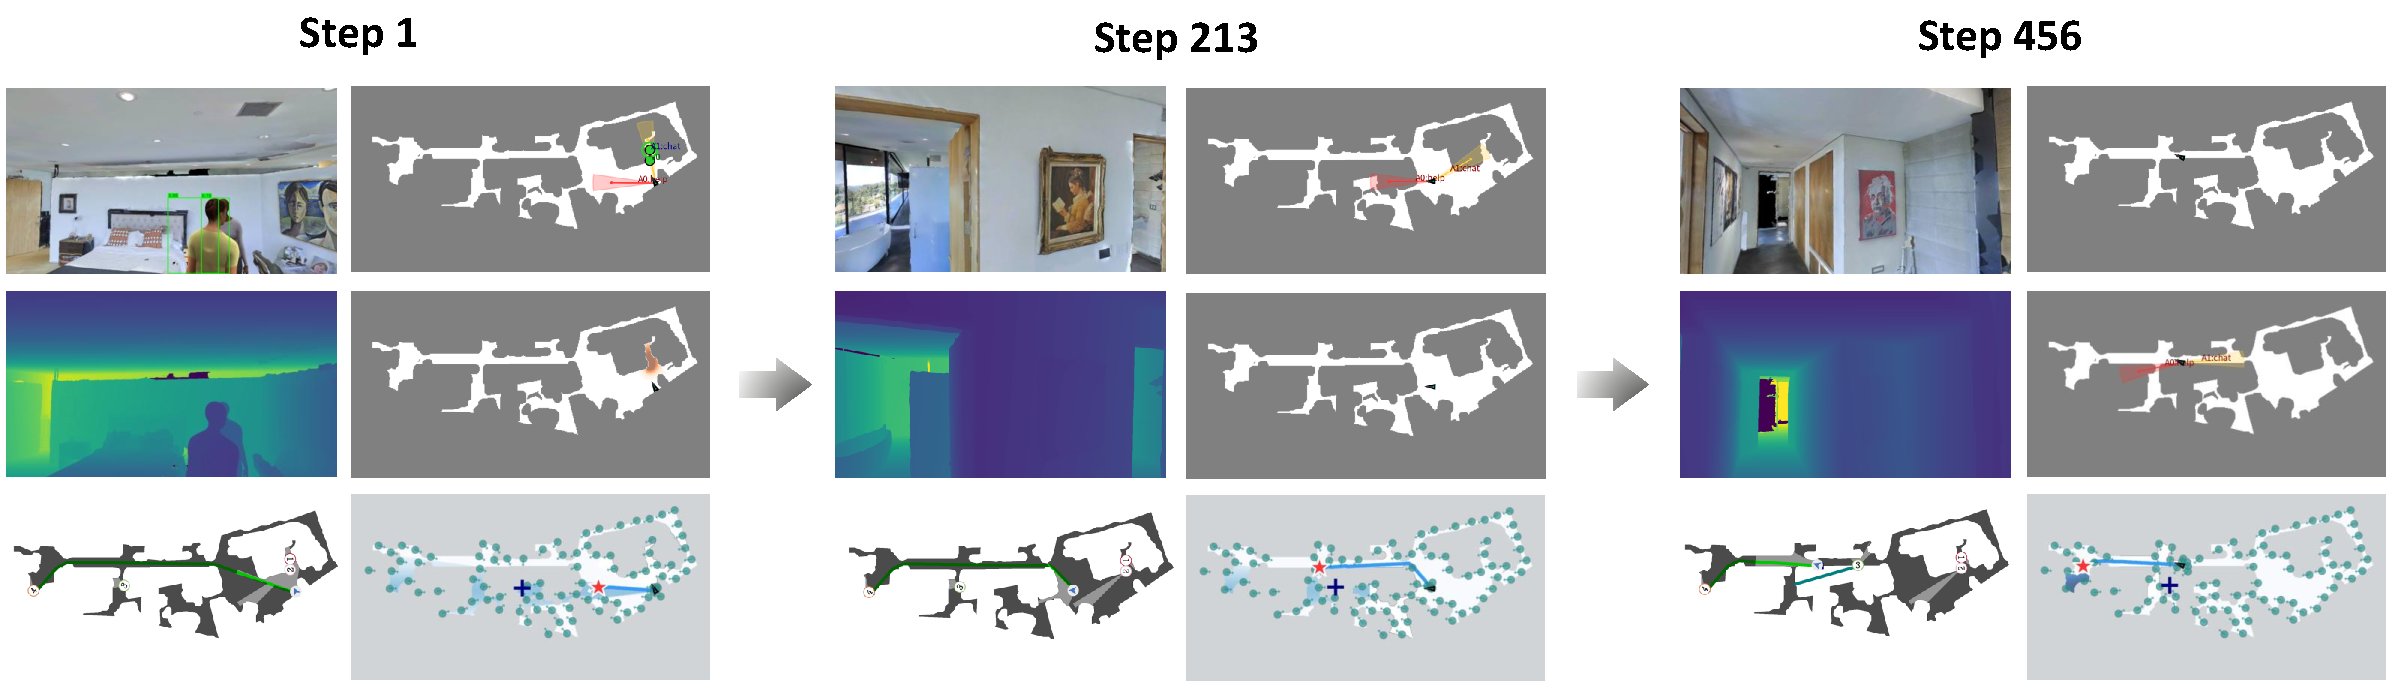
\includegraphics[width=0.98\linewidth]{figures/simulation.pdf}
	\caption{Illustration of the simulation environment and episode generation protocol. The benchmark explicitly couples semantic audio targets, multi-agent human trajectories, and precise raycast-verified NLOS conditions.}
	\label{fig:benchmark_sim}
\end{figure}

\subsection{Evaluation Metrics}
\label{subsec:benchmark-metrics}

We evaluate the navigation system across three dimensions: task completion, human safety, and social compliance. Notably, reaching the target does not inherently imply safety, necessitating distinct social metrics.

\textbf{1. Task Completion:}
\begin{itemize}
    \item \textbf{Success Rate (SR):} An episode is strictly defined as a success if the agent executes the \texttt{STOP} action within the maximum allowable time steps ($T_{max}=600$) and its final distance to the target source is $\le 1.0\,\mathrm{m}$. (Collisions do not terminate the episode, isolating navigation capability from safety).
    \item \textbf{Success weighted by Path Length (SPL):} Evaluates navigation efficiency relative to the shortest traversable path, penalizing unnecessary detours.
\end{itemize}

\textbf{2. Human Safety:}
\begin{itemize}
    \item \textbf{Human Collision Rate (HCR):} The fraction of episodes where the robot collides with a human agent. This isolates critical human-robot collisions from minor static environmental bumps.
    \item \textbf{NLOS Collision Rate (NCR):} The fraction of human collisions that occur \emph{before} or \emph{within 1.0 second} of the robot establishing direct visual observation of the human. This explicitly measures the failure to map acoustic cues into spatial awareness at blind corners.
\end{itemize}

\textbf{3. Social Compliance:}
\begin{itemize}
    \item \textbf{Personal Space Violation (PSV):} The rate at which the robot breaches the social comfort zone of any human. This unified metric applies to both moving humans ($0.8\,\mathrm{m}$ dynamic proxemics) and stationary conversational groups ($1.2\,\mathrm{m}$ static interaction zones), capturing the total duration of social intrusions relative to the episode length.
\end{itemize}

\subsection{Comparison with Existing Benchmarks}
\label{subsec:benchmark-compare}

Table~\ref{tab:benchmark_comparison} positions SAVNav against existing embodied AI paradigms. Standard Audio-Visual (AV) navigation evaluates finding a sound but ignores the social semantics of human-generated audio. Conversely, vision-based Social Navigation evaluates behavior around humans but assumes line-of-sight visibility. Moreover, emergency detection benchmarks like HomeEmergency evaluate audio-based exploration but lack explicit social compliance with active human dynamics. SAVNav bridges this gap. The agent is evaluated not merely on reaching a destination, but on its ability to \emph{hear social boundaries}---using audio to anticipate and respect human activities even when they are fully occluded.

\begin{table*}[t]
	\centering
	\caption{Comparison of SAVNav with representative embodied navigation tasks. SAVNav uniquely requires semantic audio targeting combined with NLOS social compliance.}
	\label{tab:benchmark_comparison}
	\begin{tabular}{lcccccc}
		\toprule
		Task & Goal Modality & Human Dynamics & Social Compliance & Spatial Audio & NLOS Social Risk & Semantic Targets \\
		\midrule
		ObjectNav & Vision & No & No & No & No & No \\
		SocialNav~\cite{CognitionPrecognitionFutureaware2025} & Vision & Yes & Yes & No & No & No \\
		AudioGoal~\cite{AudiovisualNavigationNoisy2025} & Audio-Visual & No & No & Yes & No & Partial \\
		HomeEmergency~\cite{HomeEmergencyUsingAudio2025} & Audio-Visual & No & No & Yes & No & Yes \\
		\textbf{SAVNav (Ours)} & \textbf{Audio-Visual} & \textbf{Yes} & \textbf{Yes} & \textbf{Yes} & \textbf{Yes} & \textbf{Yes} \\
		\bottomrule
	\end{tabular}
\end{table*}
